%
% main.tex -- Paper zum Thema SGWT
%
% (c) 2019 Hochschule Rapperswil
%

% !TeX spellcheck = de_CH_frami

\newcommand*{\laplaceL}{\ensuremath{\mathcal{L}}}
\newcommand*{\laplaceLnorm}{\ensuremath{\mathcal{L}^{\text{norm}}}}
\newcommand*{\degreeM}{\ensuremath{D}}
\newcommand*{\adjacencyM}{\ensuremath{A}}
\newcommand*{\diag}[1]{\ensuremath{\text{diag}(#1)}}


\chapter{Spectral Graph Wavelet Transform\label{chapter:sgwt}}
\lhead{SGWT}

\begin{refsection}
\chapterauthor{Hansruedi Patzen}

% !TeX spellcheck = de_CH_frami

Die Analyse und sp\"atere Synthese von Funktionen ist ein wichtiges 
mathematisches Instrument, das bei vielen Problemen eingesetzt wird. Die 
Fourier- und die Wavelet-Theorie geh\"oren dabei zu den prominentesten Methoden.

F\"ur viele Probleme lassen sich nur schwer kontinuierliche Funktionen finden, 
die den vorhanden Sachverhalt genau wiedergeben. In der heutigen digitalen Zeit 
liegen die Daten meist nur in diskreter Form vor und m\"ussen, beziehungsweise 
k\"onnen, nur so weiterverarbeitet werden.

F\"ur die Analyse und Synthese brauchen wir jeweils Basisfunktionen, mit denen 
wir die Transformation und sp\"atere R\"ucktransformation durchf\"uhren 
k\"onnen. F\"ur
Funktionen mit eindimensionalem Definitionsbereich $f: \mathbb{R} \rightarrow 
\mathbb{R}$ stellen die Exponentialfunktion $e^{i2\pi\omega x}$ eine m\"ogliche 
Basis dar, welche meist in der klassischen Fourier-Theorie verwendet wird. Im 
zweidimensionalen Fall $f: \mathbb{R}^2 \rightarrow \mathbb{R}$, wie 
beispielsweise einem Bild, wird oft eine eindimensionale
Transformation f\"ur jeweils eine Dimension vorgenommen. Man erh\"alt dann 
Basisfunktionen der Form $e^{i2\pi(ux+vy)}$. F\"ur drei Dimensionen $f: 
\mathbb{R}^3 \rightarrow \mathbb{R}$, wie zum Beispiel unsere Erdatmosph\"are 
oder auch f\"ur die zweidimensionale kosmische Mikrowellenhintergrundstrahlung, 
gibt es die Kugelfunktionen $Y^m_l$, welche eine Basis darstellen.

\begin{figure}
    \centering
    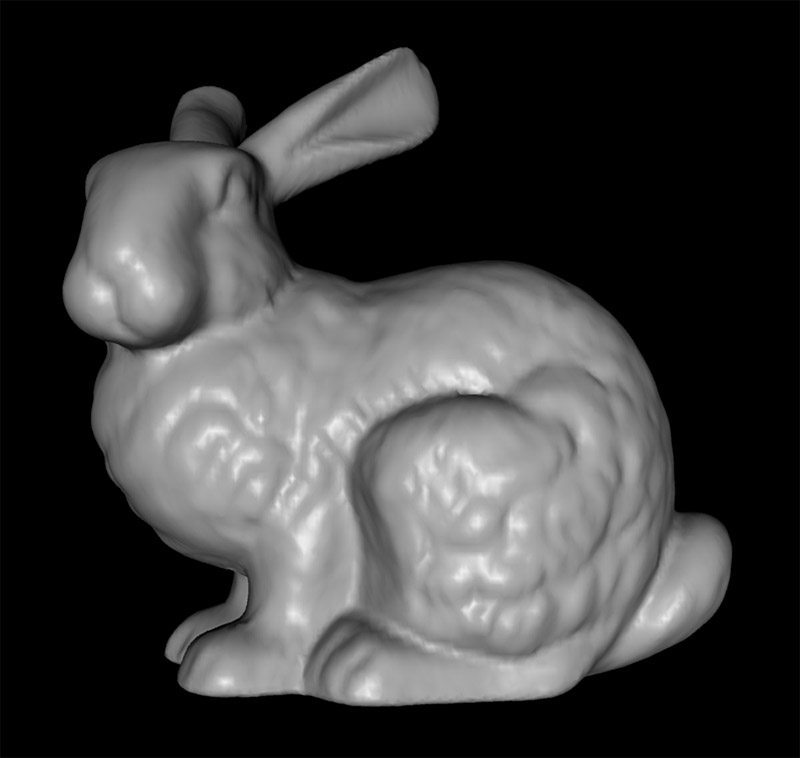
\includegraphics[
    scale=0.3
    ]{papers/sgwt/images/bunny-scanalyze-sh.jpg}
    \caption{Der Standford Bunny~\cite{noauthor_stanford_nodate} ist eines der 
    bekanntesten Testmodelle, wenn es um Computergraphiken geht.
        \label{fig:sgwt:intro:bunny}}
\end{figure}

Was ist nun aber mit Funktionen, die nicht auf einfachen K\"orperoberfl\"achen 
liegen? Zum Beispiel Funktionen auf der Oberfl\"ache des ber\"uhmten 
``Standford Bunnys''~\cite{noauthor_stanford_nodate}, zu sehen in 
\cref{fig:sgwt:intro:bunny}, welches oft als Testmodell f\"ur Computergraphiken 
eingesetzt wird. Oder bei Modellen, deren unterliegende Oberfl\"ache keine oder 
nur eine nebens\"achliche Rolle spielt, wie bei Routernetzwerken, 
Strassennetzen oder ganz generell, wenn wir nur einen Graphen haben?

In diesem Kapitel wollen wir deshalb eine Theorie entwickeln, wie 
wir die bereits bekannte Fourier- und Wavelet-Theorie auch auf einem Graphen 
anwenden 
k\"onnen, auf dessen Knoten die Funktionswerte definiert sind. Diese Theorie 
ist bekannt als ``Spectral Graph Wavelet Transform'' oder kurz SGWT -- nicht zu 
verwechseln mit der ``Second Generation Wavelet 
Transform''~\cite{noauthor_second-generation_2018}, deren K\"urzel ebenfalls 
SGWT lautet -- die erstmals 2009 in ``Wavelets on Graphs via Spectral Graph 
Theory''~\cite{hammond_wavelets_2009} vorgestellt wurde.

Wir starten mit einigen Grundlagen \"uber Graphen in~\cref{sec:sgwt:graphs} und 
gehen dann zu Laplace Operator und Matrix in~\cref{sec:sgwt:laplace} \"uber. 
Danach schauen wir uns in~\cref{sec:sgwt:spectralanalysis} die Spektralanalyse 
von Graphen genauer an und landen schlussendlich in~\cref{sec:sgwt:wavelets}, 
wo wir dann alles f\"ur die Spektral Graph Wavelet Transformation zusammen 
haben.

% !TeX spellcheck = de_CH_frami

\section{Graphen\label{sec:sgwt:graphs}}
\rhead{Graphen}

Unsere Grundlage, auf der wir die SGWT aufbauen wollen, stellen Graphen dar. 
Ein Graph $G$ setzt sich aus Kanten $E$ und Knoten $V$ zusammen.
\begin{equation*}
G = \{V, E\}
\end{equation*}
Eine Kante verbindet dabei jeweils zwei Knoten miteinander.
\begin{equation*}
E \subset \{\{v_1, v_2\} | v_i \in V, v_1 \neq v_2 \}
\end{equation*}

\begin{figure}
    \centering
    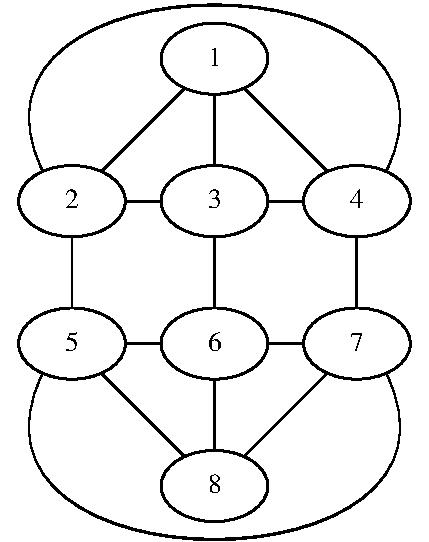
\includegraphics[
        scale=0.7
    ]{papers/sgwt/images/sphere-graph.pdf}
    \caption{Graph Approximation einer Kugel.
    \label{fig:sgwt:sphere:graph}}
\end{figure}

\begin{figure}
    \centering
    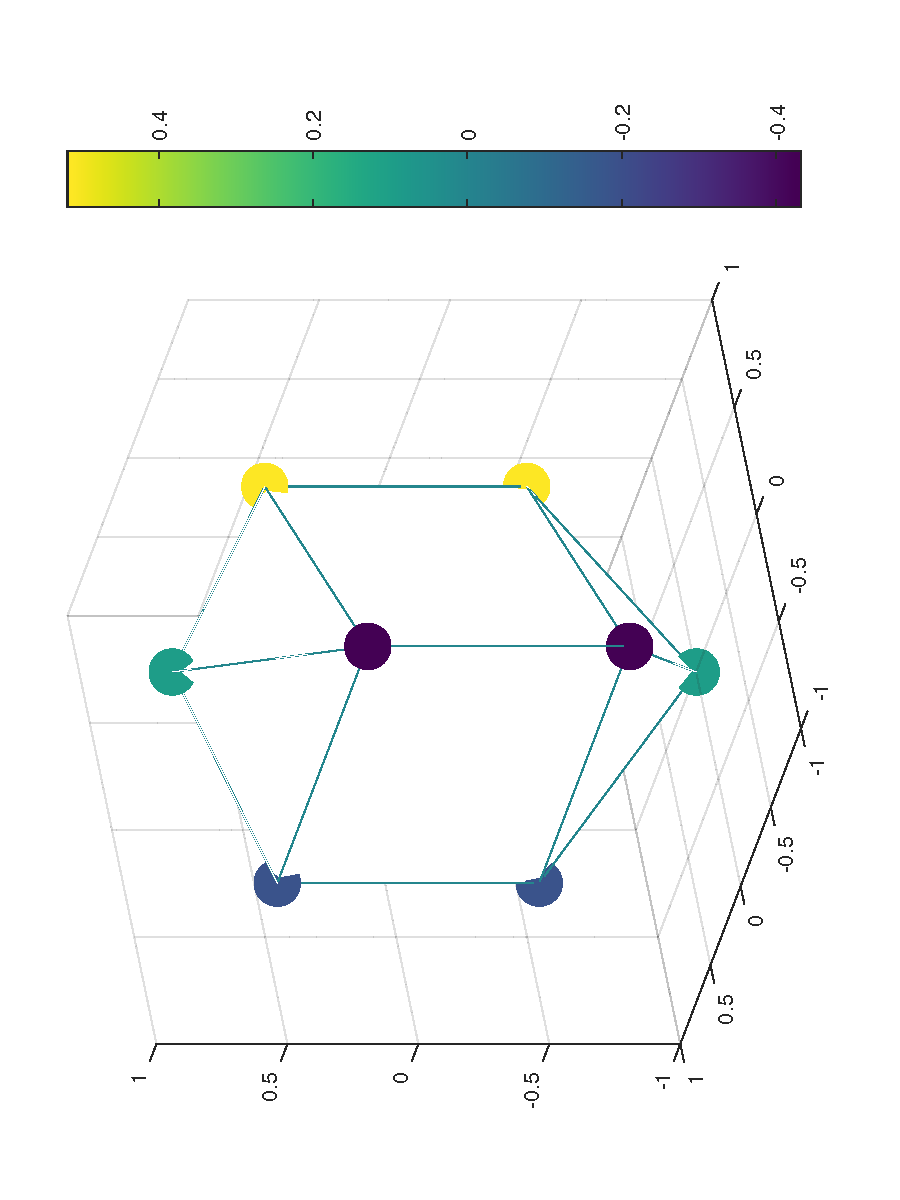
\includegraphics[
        angle=-90,
        origin=c,
        scale=0.7
    ]{papers/sgwt/images/graph-chi-4.pdf}
    \vspace{-80pt}
    \caption{Dreidimensionale Darstellung des Kugelgraphen. Die Funktionswerte 
    werden dabei mit Farben auf den Knoten dargestellt. 
    \label{fig:sgwt:sphere:graph:chi}}
\end{figure}

\begin{figure}
    \centering
    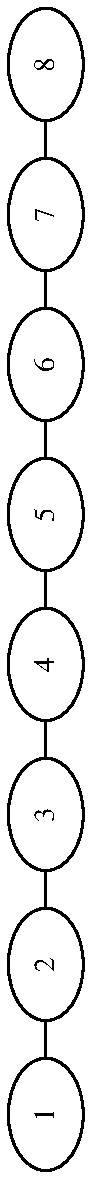
\includegraphics[
        angle=-90,
        origin=c,
        scale=0.7
    ]{papers/sgwt/images/line-graph.pdf}
    \vspace{-200pt}
    \caption{Graph Approximation einer eindimensionalen Funktion. 
    \label{fig:sgwt:line:graph}}
\end{figure}

\begin{figure}
    \centering
    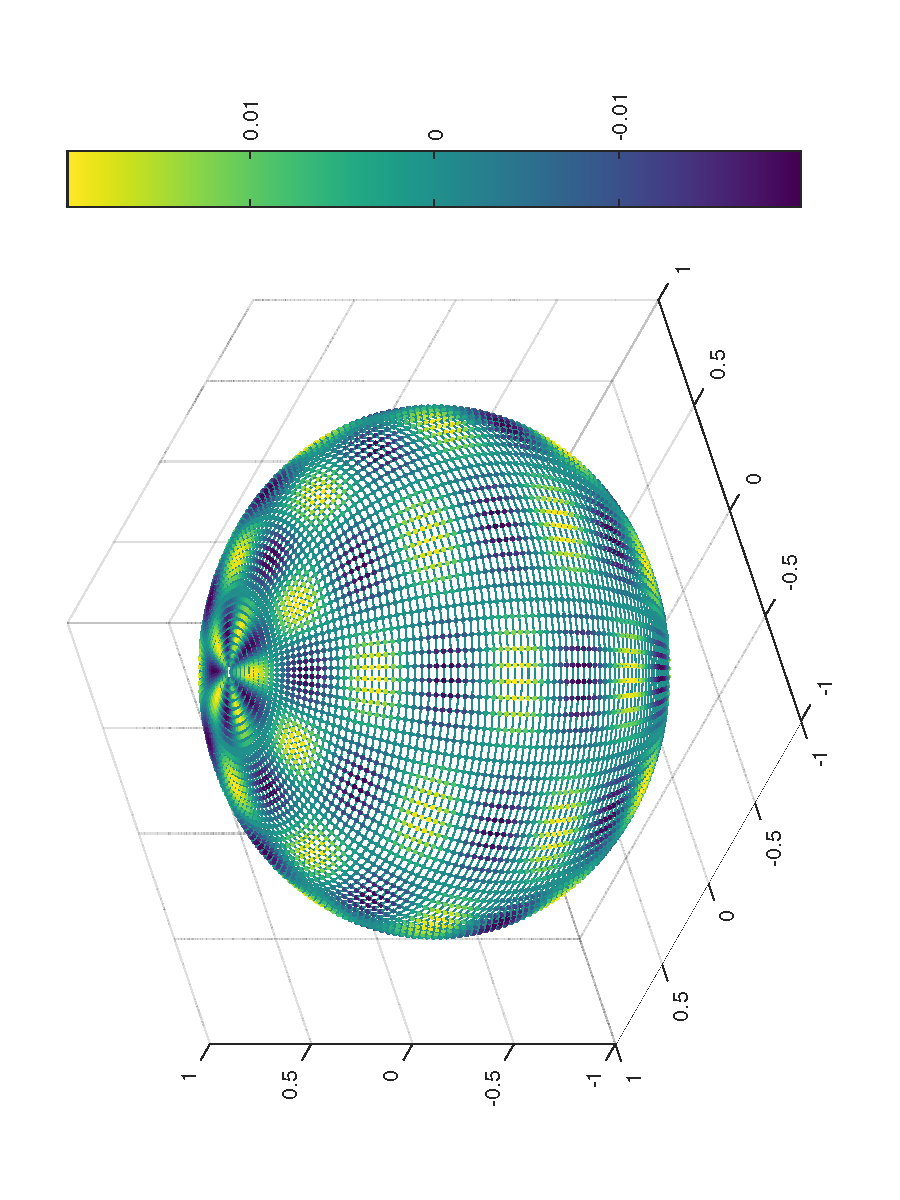
\includegraphics[
        angle=-90,
        origin=c,
        scale=0.7
    ]{papers/sgwt/images/graph-100-100-chi-150.pdf}
    \vspace{-80pt}
    \caption{Kugelgraph mit $l = b = 100$. Darstellung von $\chi_{150}$.
    \label{fig:sgwt:sphere:graph:chi:hh}}
\end{figure}

\begin{figure}
    \centering
    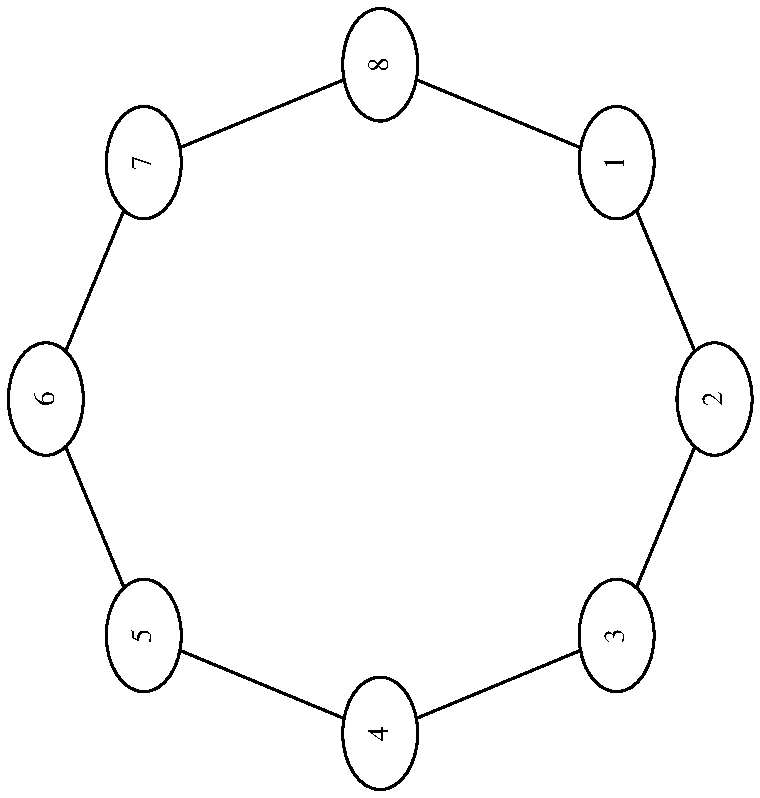
\includegraphics[
        angle=-90,
        origin=c,
        scale=0.7
    ]{papers/sgwt/images/ring-graph.pdf}
    \caption{Graph Approximation einer periodischen eindimensionalen Funktion. 
    \label{fig:sgwt:ring:graph}}
\end{figure}


\section{Laplace\label{sec:sgwt:laplace}}
\rhead{Laplace}

\subsection{Laplace Operator\label{subsec:sgwt:laplaceop}}
\rhead{Laplace Operator}

Der Laplace operator $\Delta$ in $\mathbb{R}^n$ beschreibt die zweite Ableitung.

\begin{equation}
\Delta = \frac{\partial^2}{\partial x_1^2}
+ \frac{\partial^2}{\partial x_2^2}
+ \dots
+ \frac{\partial^2}{\partial x_n^2}
\end{equation}

\subsection{Laplace Matrix\label{subsec:sgwt:laplacm}}
\rhead{Laplace Matrix}

%TODO: Why could norm be usefull?

%TODO: Rework
Die Laplace Matrix 
\laplaceL~\cite{noauthor_laplace-matrix_2017}, welche wir aus der 
Gradmatrix \degreeM~\cite{noauthor_degree_2018} und der Adjazenzmatrix 
\adjacencyM~\cite{noauthor_adjacency_2019} berechnen k\"onnen, spielt bei der 
SGWT eine entscheidende Rolle. Dabei gibt es 
die Unterscheidung zwischen der Laplace Matrix aus \cref{eq:sgwt:laplace} und 
\cref{eq:sgwt:laplace:norm}, bei der \laplaceLnorm{} Matrix handelt es sich um 
die normalisierte \laplaceL{} Matrix.

\begin{equation}
\laplaceL = \degreeM - \adjacencyM
\label{eq:sgwt:laplace}
\end{equation}

\begin{equation}
\laplaceLnorm
= \degreeM^{-1/2}\laplaceL\degreeM^{-1/2}
= I - \degreeM^{-1/2}\adjacencyM\degreeM^{-1/2}
\label{eq:sgwt:laplace:norm}
\end{equation}

\begin{equation}
\chi = 
\left[
\begin{pmatrix}\\\chi_0\\\\\end{pmatrix}
\begin{pmatrix}\\\chi_1\\\\\end{pmatrix}
\begin{pmatrix}\\\chi_2\\\\\end{pmatrix}
\cdots
\begin{pmatrix}\\\chi_{N-1}\\\\\end{pmatrix}
\right]
\end{equation}

\begin{equation}
0 = \lambda_0 < \lambda_1 \le \lambda_2 \le \cdots \le \lambda_{N-1}
\end{equation}

% !TeX spellcheck = de_CH_frami

\section{Graph Spektralanalyse\label{sec:sgwt:spectralanalysis}}
\rhead{Graph Spektralanalyse}

Nachdem wir nun die Grundlagen von Graphen und den Laplace Operator sowie die 
Laplace Matrix angeschaut haben, wollen wir uns nun der Spektralanalyse eines 
Graphen widmen.

\subsection{Laplace Matrix Eigenwerte}

Wenn man vom Spektrum eines Graphen spricht, meint man damit die Eigenwerte 
$\lambda$ seiner Laplace Matrix. Da diese Matrix bei einem ungerichteten 
Graphen immer symmetrisch ist, werden die daraus folgenden Eigenwerte und 
Eigenfunktionen auch immer real und gr\"osser gleich $0$ sein. Es gilt somit
\begin{equation}
0 = \lambda_0 < \lambda_1 \leq \lambda_2 \leq \cdots \leq \lambda_{N-1}.
\label{eq:sgwt:lambda:series}
\end{equation}
\Cref{fig:sgwt:lambda:line} zeigt die Eigenwerte $\lambda_0$ bis 
$\lambda_{999}$ eines Ringraphen mit 1000 Knoten.

\begin{figure}
    \centering
    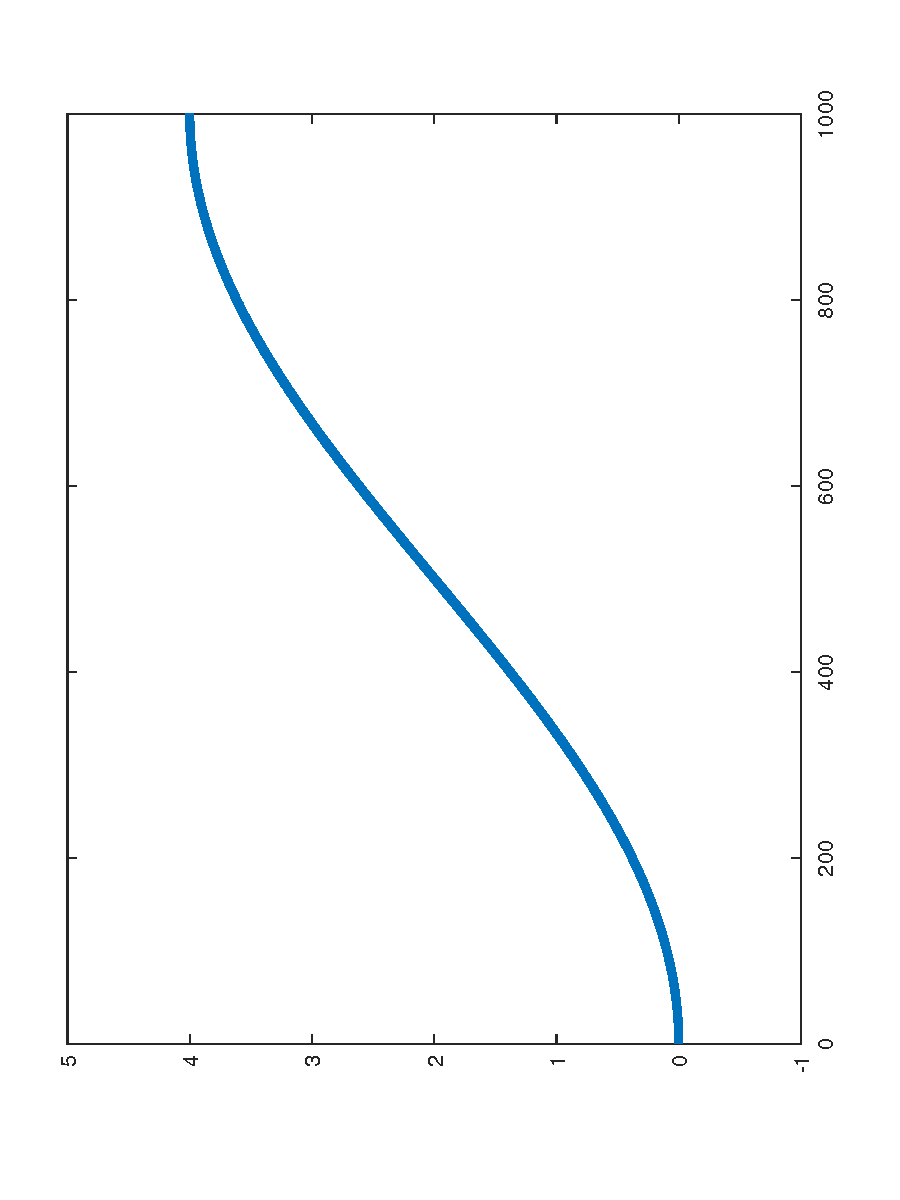
\includegraphics[
    angle=-90,
    origin=c,
    scale=0.6
    ]{papers/sgwt/images/ring-lambda.pdf}
    \vspace{-70pt}
    \caption{$\lambda_0$ bis $\lambda_{999}$ eines nicht gewichteten Ringraphen.
        \label{fig:sgwt:lambda:line}}
\end{figure}

\subsection{Laplace Matrix Eigenvektoren}

Eine weitere wichtige Rolle spielen die Eigenvektoren der Laplace Matrix. Diese 
sind n\"amlich approximierte Eigenfunktionen des Laplace Operators $\Delta$. So 
ist die komplexe Exponentialfunktion $e^{i\omega x}$ die Eigenfunktion des 
eindimensionalen Laplace Operators 
$\frac{d^2}{dx^2}$~\cite{chung_spectral_nodate}. Dies wird deutlich, wenn 
wir die Eigenfunktionen eines 
Ring-,~\cref{fig:sgwt:chi:ring0,fig:sgwt:chi:ring1,fig:sgwt:chi:ring2,fig:sgwt:chi:ring3,fig:sgwt:chi:ring4,fig:sgwt:chi:ring5},
oder 
Liniengraphen,~\cref{fig:sgwt:chi:line0,fig:sgwt:chi:line1,fig:sgwt:chi:line2,fig:sgwt:chi:line3,fig:sgwt:chi:line4,fig:sgwt:chi:line5},
darstellen. Auch die Kugelfunktionen $Y^m_l$, lassen mit den Hilfe der 
Eigenfunktionen eines Kugelgraphen approximieren, wie man 
in~\cref{fig:sgwt:chi:sphere} sehen kann. Dabei wird aber auch deutlich, dass 
diese Approximation nicht \"uberall gleich gut ist. Insbesondere dadurch, dass 
der Grad an den Polen stark von den anderen Knoten abweicht, findet dort eine 
Verzerrung statt.

\begin{figure}
\centering
\begin{minipage}[b]{0.49\textwidth}
    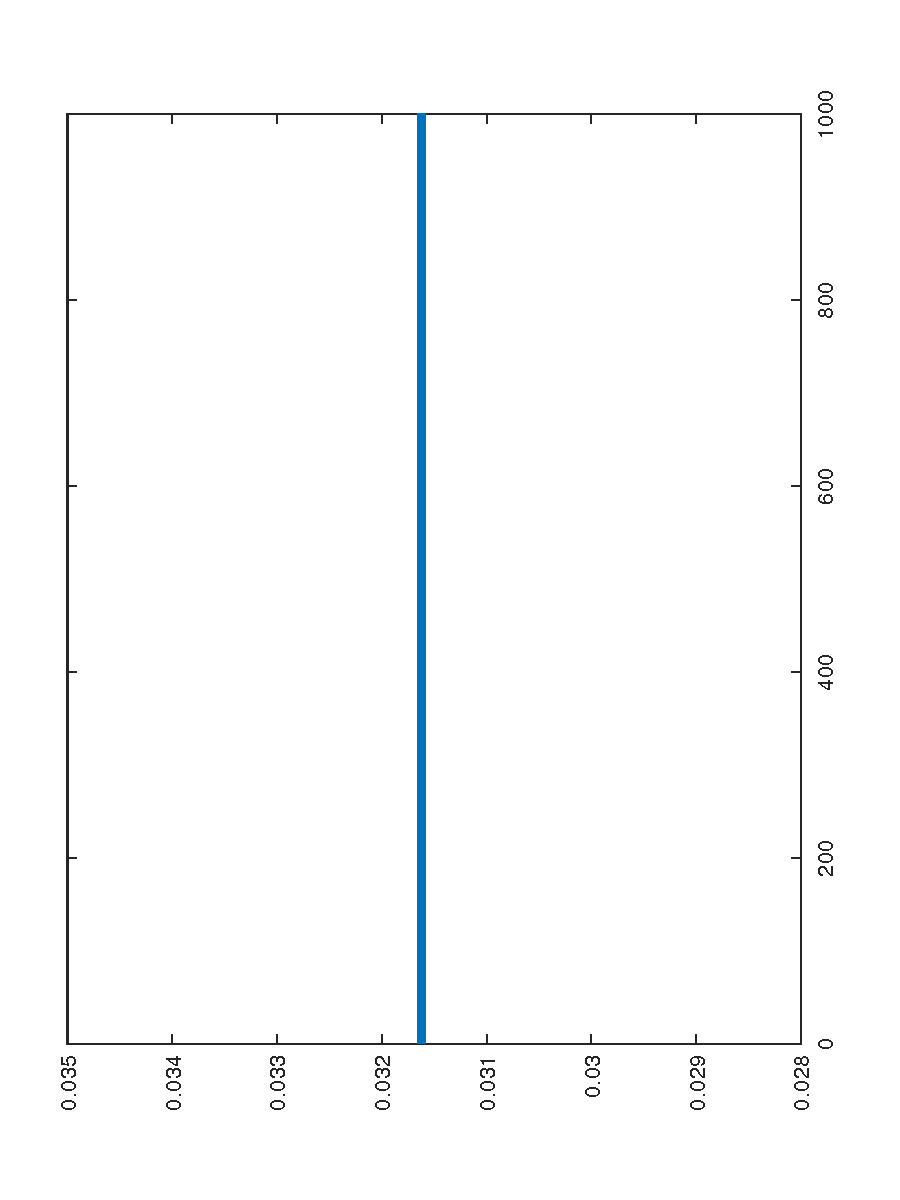
\includegraphics[
    angle=-90,
    origin=c,
    width=\textwidth]{papers/sgwt/images/ring-chi-1.pdf}
    \vspace{-45pt}
    \caption{$\chi_0$ eines ungewichteten Ringraphen mit 1000 Knoten.}
    \label{fig:sgwt:chi:ring0}
\end{minipage}
~
\begin{minipage}[b]{0.49\textwidth}
    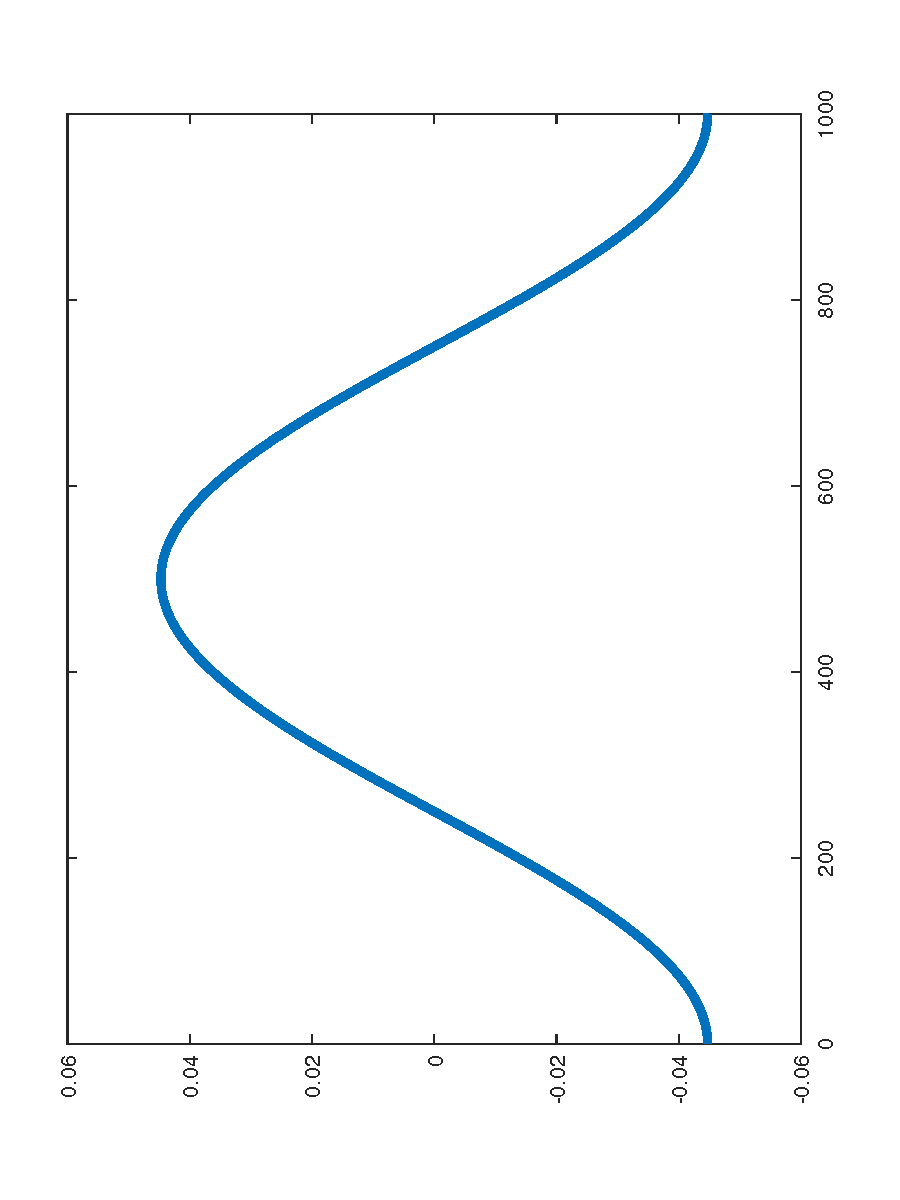
\includegraphics[
    angle=-90,
    origin=c,
    width=\textwidth]{papers/sgwt/images/ring-chi-2.pdf}
    \vspace{-45pt}
    \caption{$\chi_1$ eines ungewichteten Ringraphen mit 1000 Knoten.}
    \label{fig:sgwt:chi:ring1}
\end{minipage}
~
\begin{minipage}[b]{0.49\textwidth}
    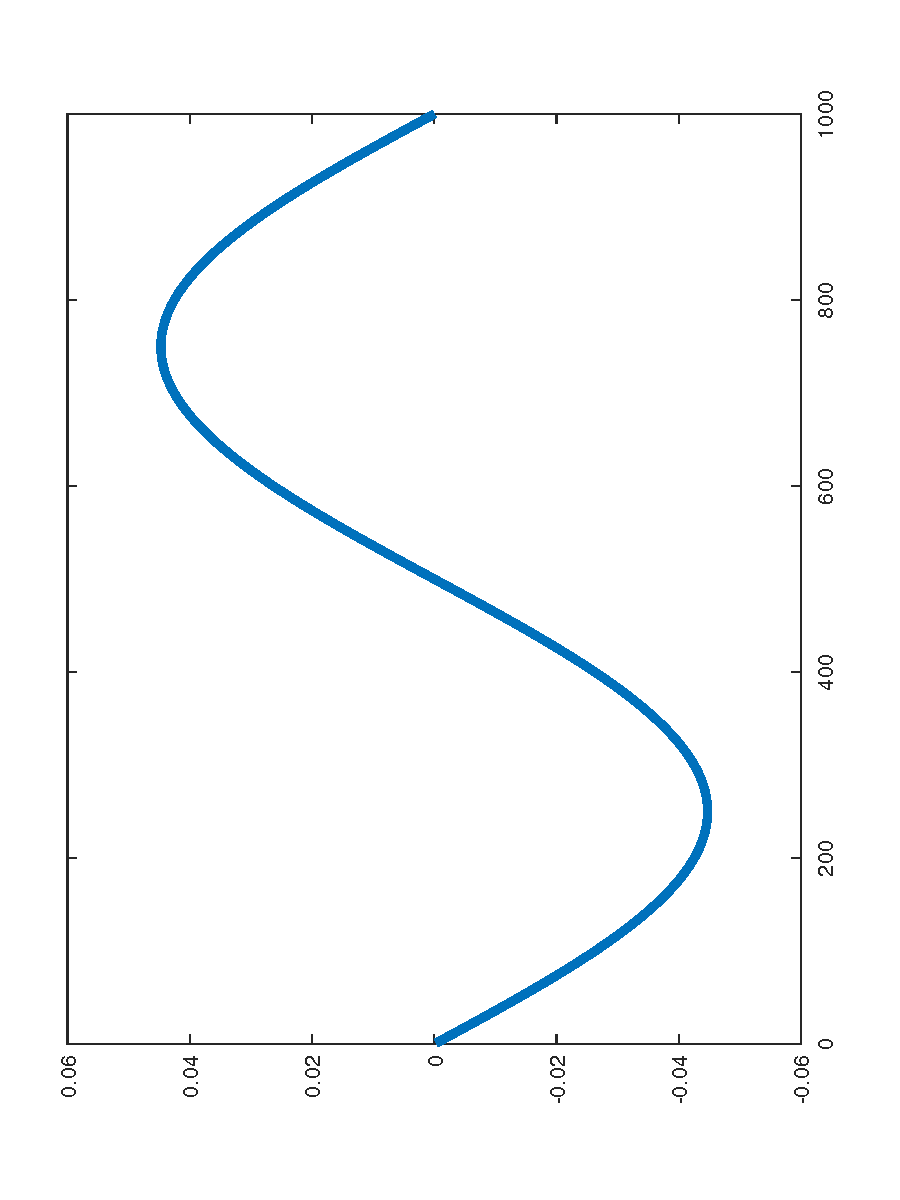
\includegraphics[
    angle=-90,
    origin=c,
    width=\textwidth]{papers/sgwt/images/ring-chi-3.pdf}
    \vspace{-45pt}
    \caption{$\chi_2$ eines ungewichteten Ringraphen mit 1000 Knoten.}
    \label{fig:sgwt:chi:ring2}
\end{minipage}
~
\begin{minipage}[b]{0.49\textwidth}
    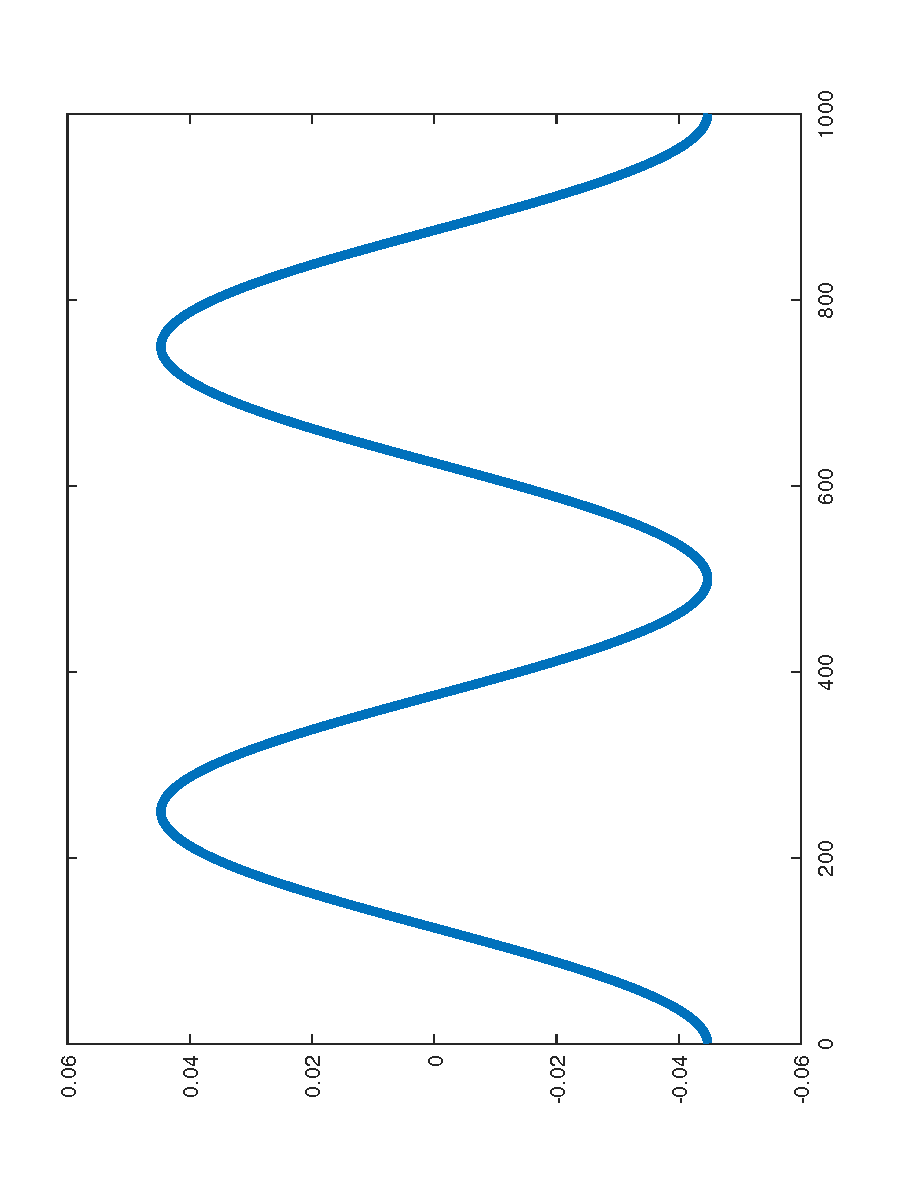
\includegraphics[
    angle=-90,
    origin=c,
    width=\textwidth]{papers/sgwt/images/ring-chi-4.pdf}
    \vspace{-45pt}
    \caption{$\chi_3$ eines ungewichteten Ringraphen mit 1000 Knoten.}
    \label{fig:sgwt:chi:ring3}
\end{minipage}
~
\begin{minipage}[b]{0.49\textwidth}
    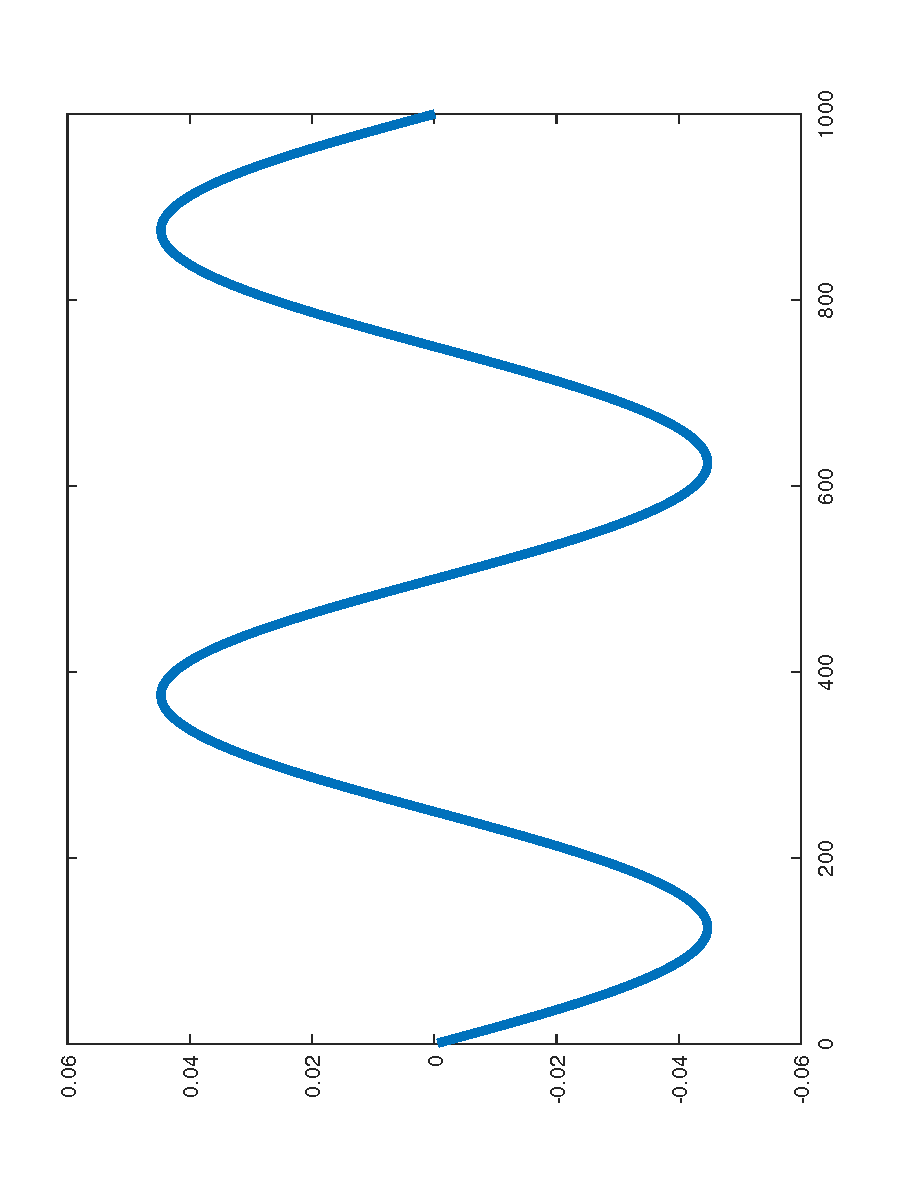
\includegraphics[
    angle=-90,
    origin=c,
    width=\textwidth]{papers/sgwt/images/ring-chi-5.pdf}
    \vspace{-45pt}
    \caption{$\chi_4$ eines ungewichteten Ringraphen mit 1000 Knoten.}
    \label{fig:sgwt:chi:ring4}
\end{minipage}
~
\begin{minipage}[b]{0.49\textwidth}
    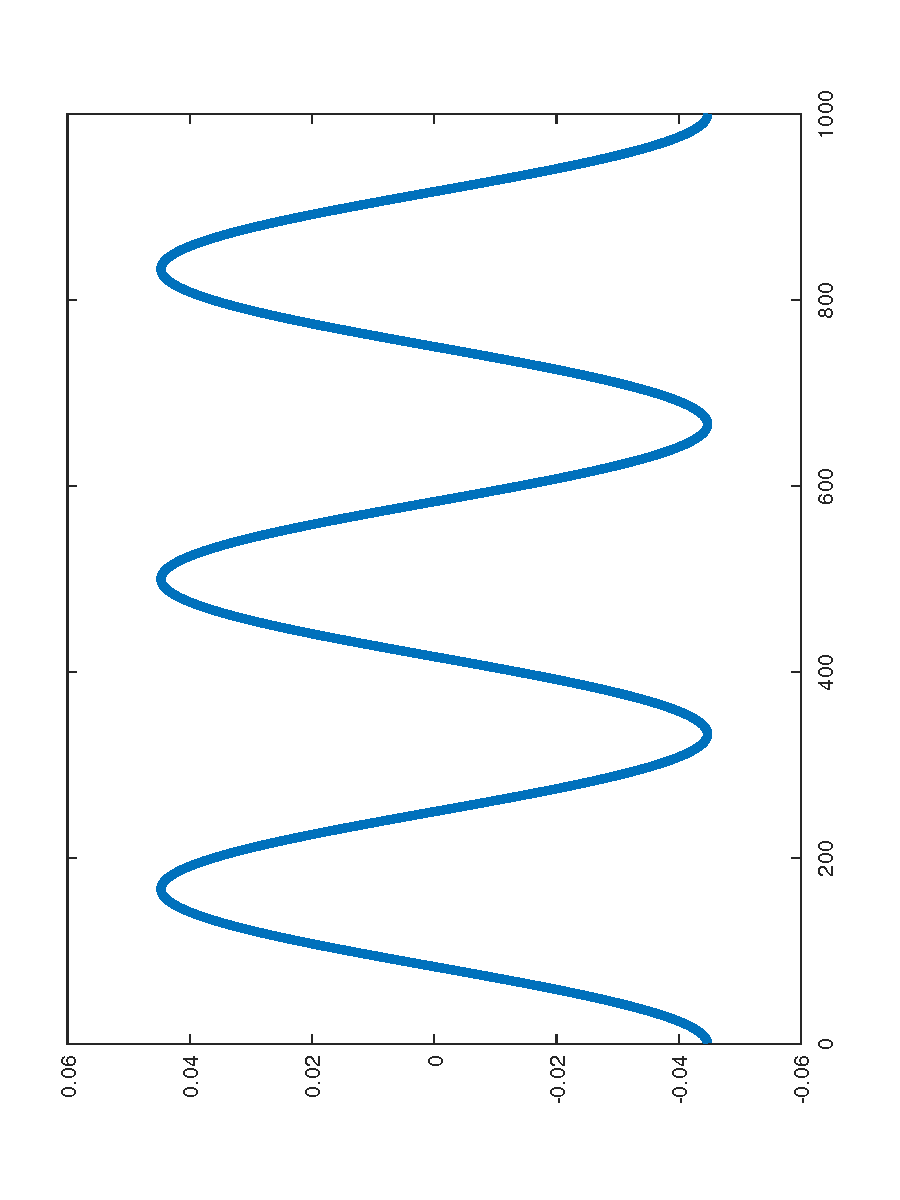
\includegraphics[
    angle=-90,
    origin=c,
    width=\textwidth]{papers/sgwt/images/ring-chi-6.pdf}
    \vspace{-45pt}
    \caption{$\chi_5$ eines ungewichteten Ringraphen mit 1000 Knoten.}
    \label{fig:sgwt:chi:ring5}
\end{minipage}
\end{figure}

\begin{figure}
    \centering
    \begin{minipage}[b]{0.49\textwidth}
        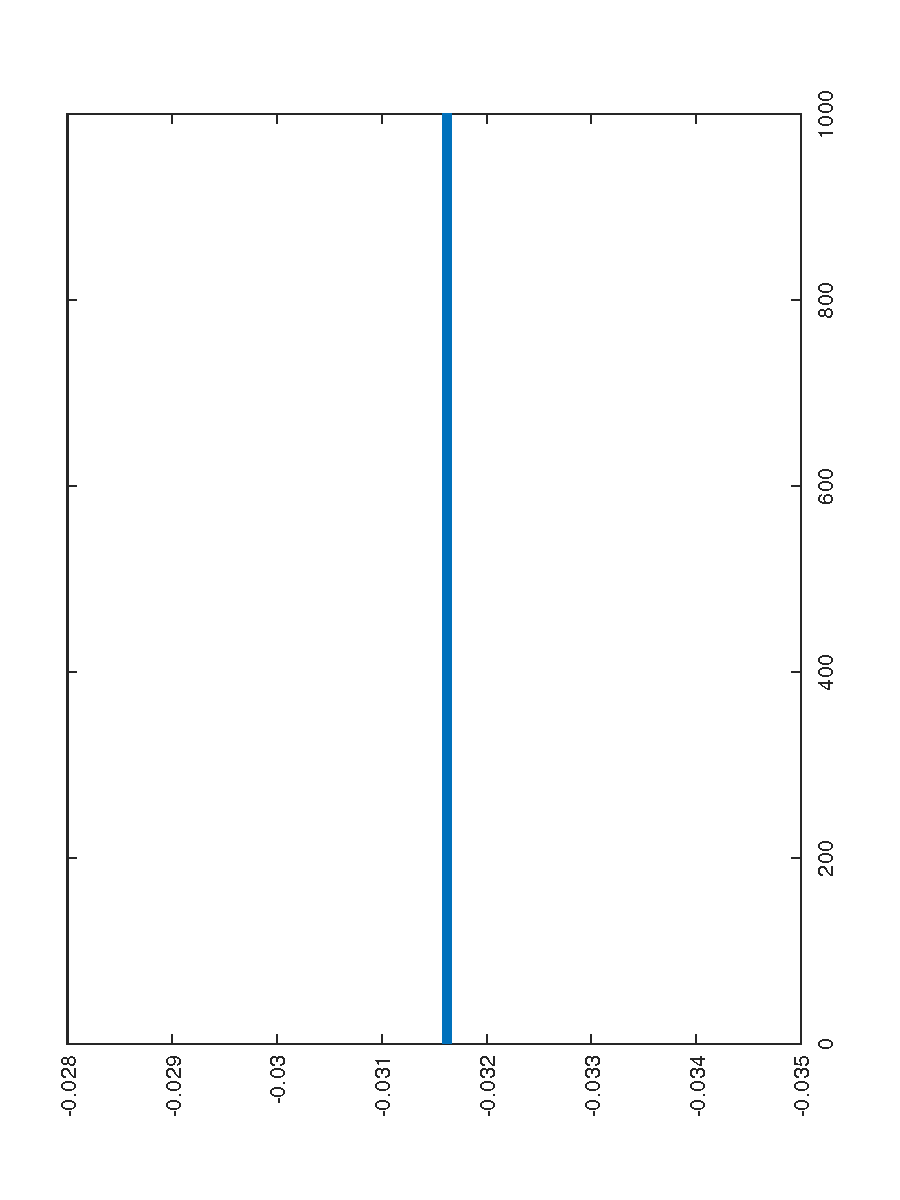
\includegraphics[
        angle=-90,
        origin=c,
        width=\textwidth]{papers/sgwt/images/line-chi-1.pdf}
        \vspace{-45pt}
        \caption{$\chi_0$ eines ungewichteten Liniengraphen mit 1000 
        Knoten.}
        \label{fig:sgwt:chi:line0}
    \end{minipage}
    ~
    \begin{minipage}[b]{0.49\textwidth}
        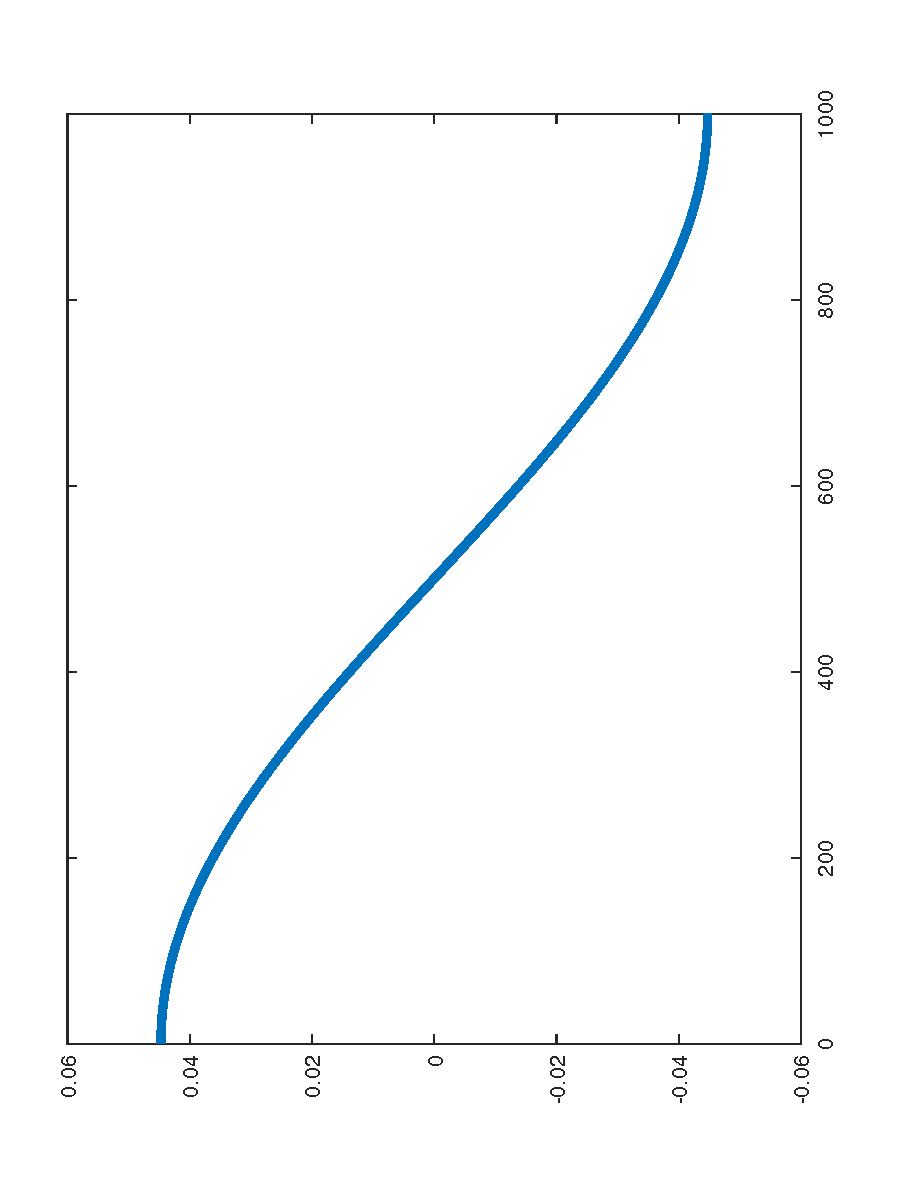
\includegraphics[
        angle=-90,
        origin=c,
        width=\textwidth]{papers/sgwt/images/line-chi-2.pdf}
        \vspace{-45pt}
        \caption{$\chi_1$ eines ungewichteten Liniengraphen mit 1000 
        Knoten.}
        \label{fig:sgwt:chi:line1}
    \end{minipage}
    ~
    \begin{minipage}[b]{0.49\textwidth}
        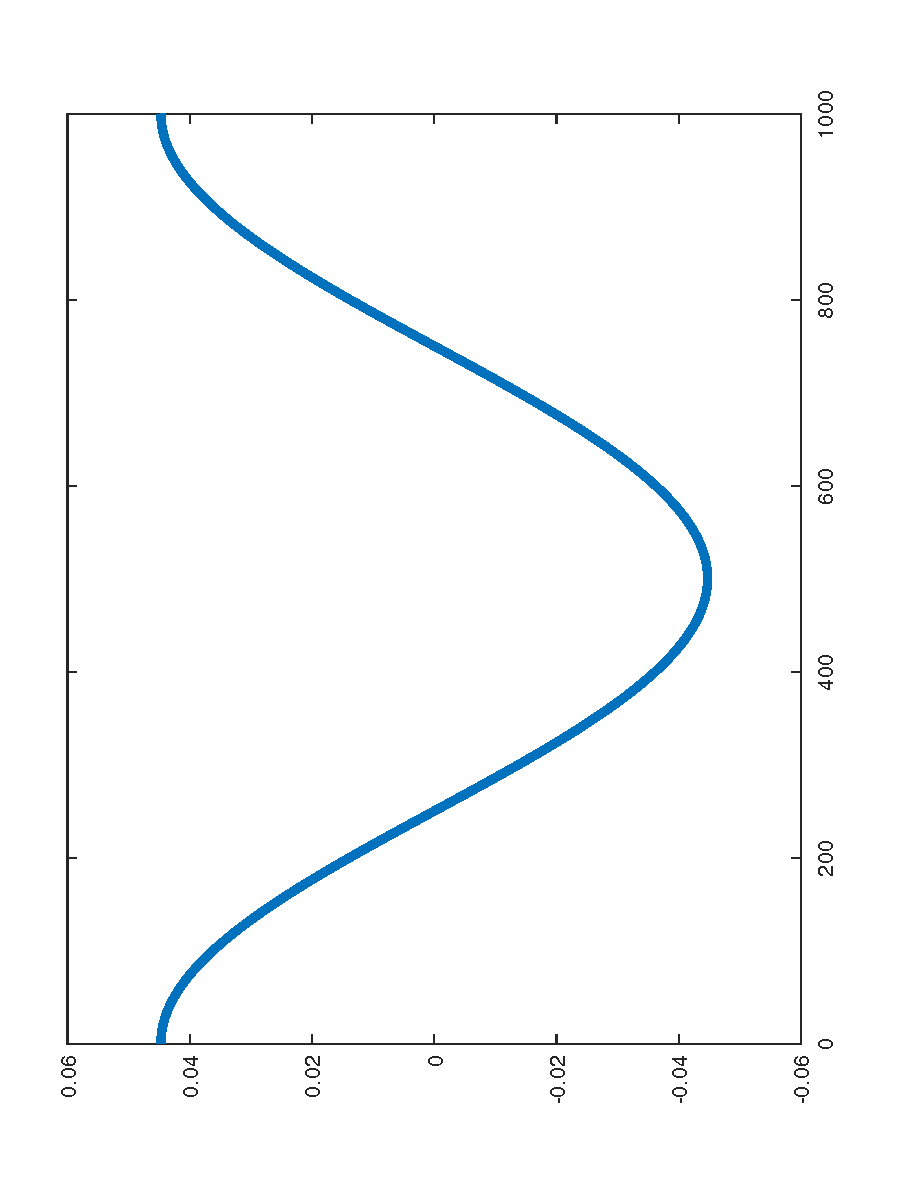
\includegraphics[
        angle=-90,
        origin=c,
        width=\textwidth]{papers/sgwt/images/line-chi-3.pdf}
        \vspace{-45pt}
        \caption{$\chi_2$ eines ungewichteten Liniengraphen mit 1000 
        Knoten.}
        \label{fig:sgwt:chi:line2}
    \end{minipage}
    ~
    \begin{minipage}[b]{0.49\textwidth}
        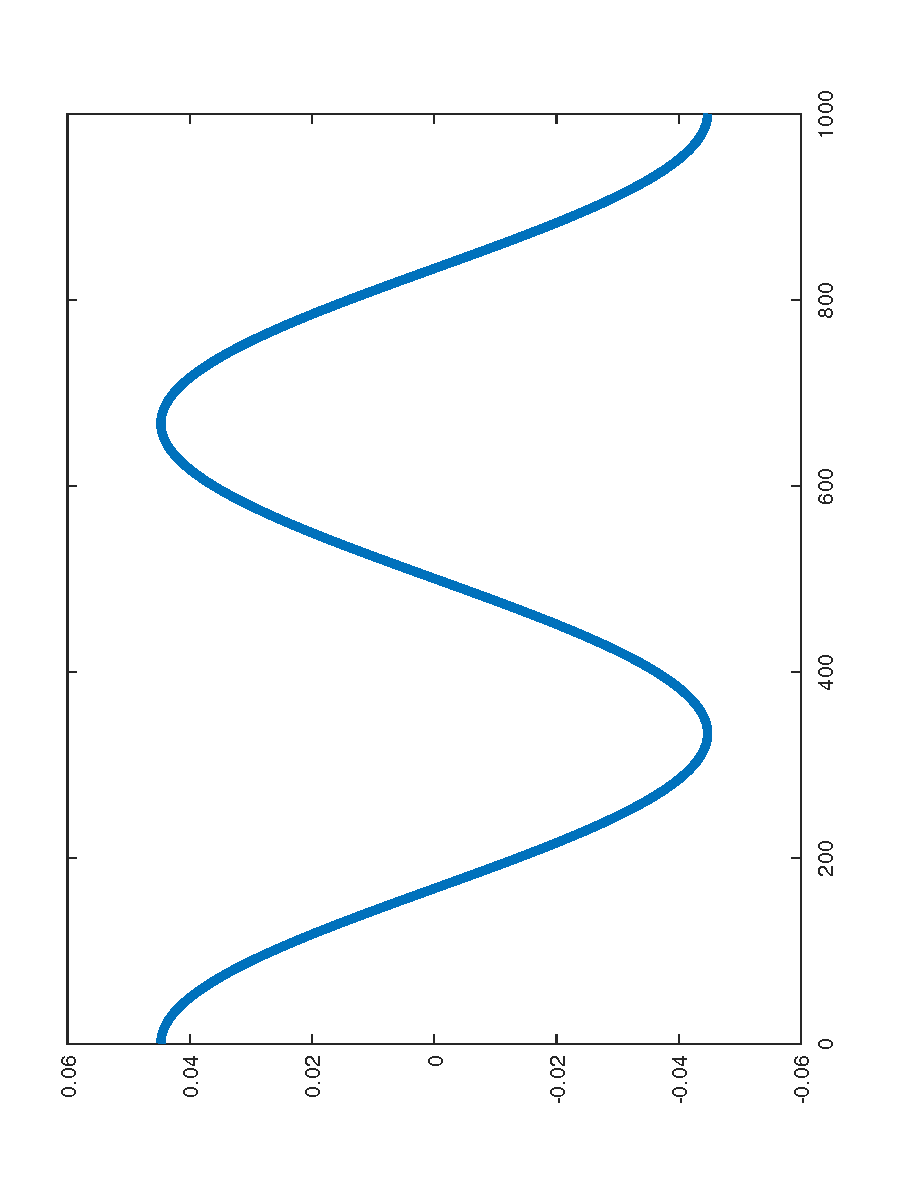
\includegraphics[
        angle=-90,
        origin=c,
        width=\textwidth]{papers/sgwt/images/line-chi-4.pdf}
        \vspace{-45pt}
        \caption{$\chi_3$ eines ungewichteten Liniengraphen mit 1000 
        Knoten.}
        \label{fig:sgwt:chi:line3}
    \end{minipage}
    ~
    \begin{minipage}[b]{0.49\textwidth}
        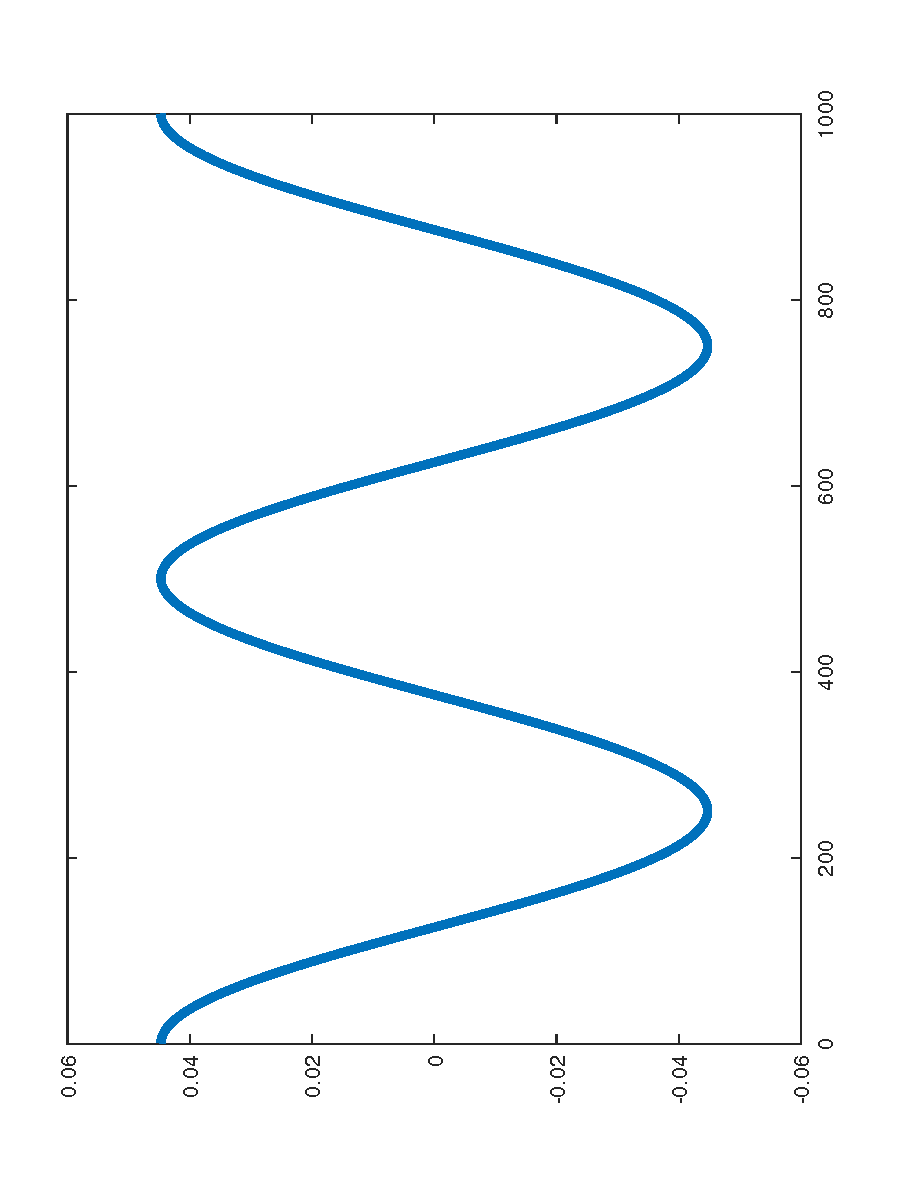
\includegraphics[
        angle=-90,
        origin=c,
        width=\textwidth]{papers/sgwt/images/line-chi-5.pdf}
        \vspace{-45pt}
        \caption{$\chi_4$ eines ungewichteten Liniengraphen mit 1000 
        Knoten.}
        \label{fig:sgwt:chi:line4}
    \end{minipage}
    ~
    \begin{minipage}[b]{0.49\textwidth}
        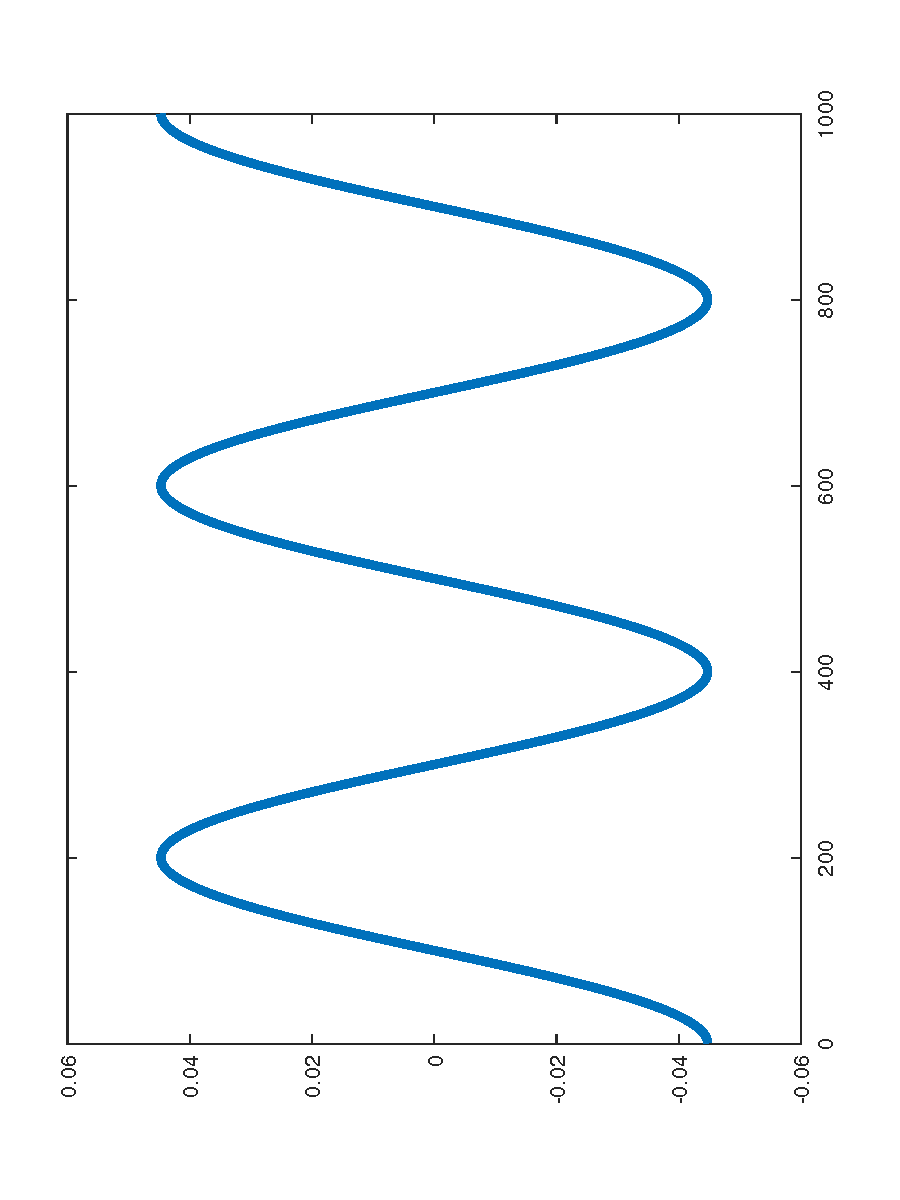
\includegraphics[
        angle=-90,
        origin=c,
        width=\textwidth]{papers/sgwt/images/line-chi-6.pdf}
        \vspace{-45pt}
        \caption{$\chi_5$ eines ungewichteten Liniengraphen mit 1000 
        Knoten.}
        \label{fig:sgwt:chi:line5}
    \end{minipage}
\end{figure}

\begin{figure}
    \centering
    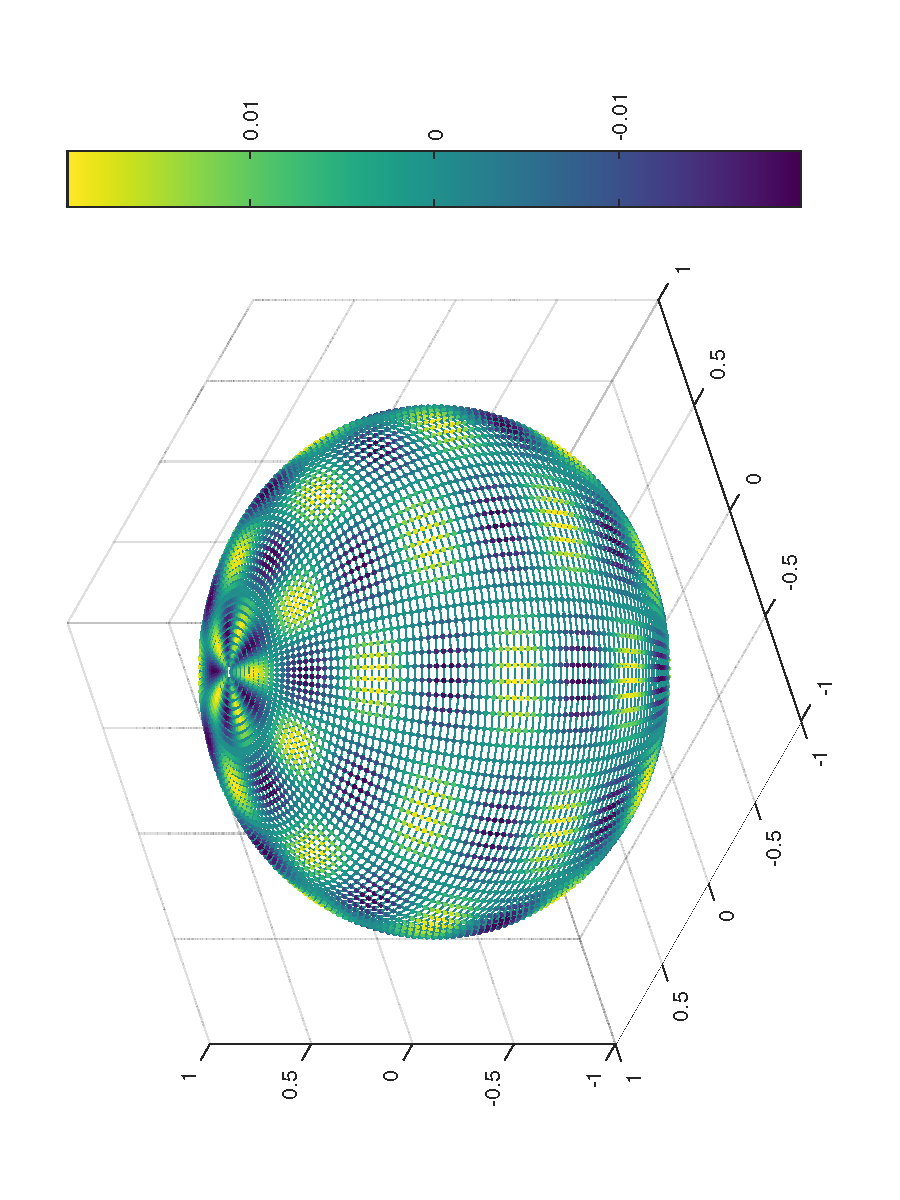
\includegraphics[
    angle=-90,
    origin=c,
    scale=0.7
    ]{papers/sgwt/images/graph-100-100-chi-150.pdf}
    \vspace{-80pt}
    \caption{Kugelgraph mit 10002 Knoten. Darstellung von $\chi_{150}$.
        \label{fig:sgwt:chi:sphere}}
\end{figure}
% !TeX spellcheck = de_CH_frami

\section{Zusammenfassung\label{sec:sgwt:summary}}
\rhead{Zusammenfassung}

Mit der Spektral Graph Wavelet Transformation ist es uns gelungen, die bekannte 
Wavelettheorie auch auf Graphen anzuwenden. Damit k\"onnen wir uns von der 
Geometrie der Oberfl\"ache einer Funktion l\"osen und betrachten nur noch, was 
in der Nachbarschaft der einzelnen Knoten geschieht.

Um nun eine Funktion $f(v)$ auf einem Graphen $G$ zu analysieren, k\"onnen wir 
also wie folgt vorgehen
\begin{itemize}
    \item[1.] Generierung der \laplaceL{} Matrix aus dem Graphen $G$.
    \item[2.] Berechnung der Eigenwerte $\lambda$ und Eigenvektoren $\chi$.
    \item[3.] Berechnung der $\psi_j$ und $\phi$ Wavelets 
    mit~\cref{eq:sgwt:psi,eq:sgwt:phi}.
    \item[4.] Berechnung der Wavelet Koeffizienten $\hat{f}$ 
    mit~\cref{eq:sgwt:hatf}.
\end{itemize}
Danach k\"onnen wir die Funktion $f$ mittels~\cref{eq:sgwt:pseudof} wieder 
synthetisieren, indem wir das Pseudoinverse der $T$-Matrix verwenden.

Auch wenn die SGWT, im Vergleich zu zur Wavelet- oder gar Fouriertheorie noch 
ziemlich neu ist, scheinen die M\"oglichkeiten \"ausserst weitl\"aufig zu sein, 
wie Beispiele in der in der Bildbearbeitung~\cite{shuman_emerging_2013} oder 
bei der Verwendung von neuronalen Netzwerken~\cite{xu_graph_2019} zeigen.



% TODO: Remove in final version. replaces \nocite{*}.
Literatur:
\cite{noauthor_second-generation_2018}
\cite{noauthor_laplace-matrix_2017}
\cite{noauthor_degree_2018}
\cite{noauthor_adjacency_2019}
\cite{hammond_wavelets_2009}
\cite{hammond_image_nodate}
\cite{shuman_emerging_2013}
\cite{xu_graph_2019}
\cite{chung_spectral_nodate}
\cite{spielman_spectral_nodate}
\cite{nica_brief_2018}
\cite{marsden_eigenvalues_nodate}


\printbibliography[heading=subbibliography]
\end{refsection}
